\section{Secuencias}\label{sec:uc0}


\subsection{Administrador}\label{sec:uc0}
\subsubsection{Borrar partida de un usuario}
\begin{center}
	  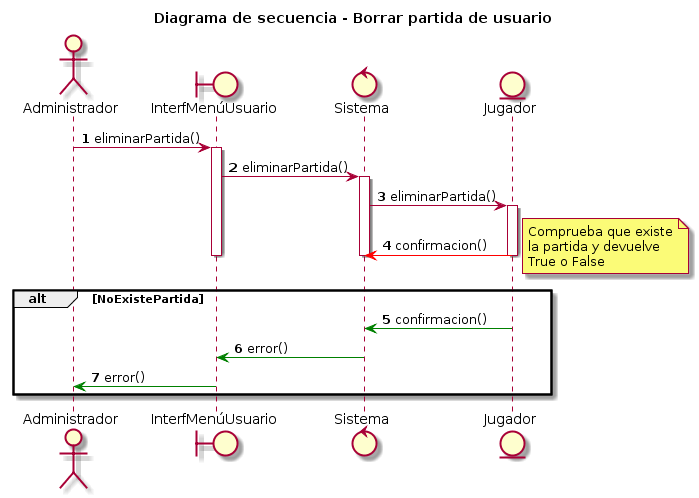
\includegraphics[width=0.9\textwidth]{./imatges/administrador/Borrar_partida_de_usuario.png}
\end{center}
Para borrar una partida, desde el administrador se llama a la función eliminarPartida hasta Jugador, donde se verificará si existe la partida o no, en el caso que exista la partida, la función devuelve al sistema True y en caso contrario False. \\
	Una vez el sistema ha recibido la confirmación, envia un error hasta el administrador.

\subsubsection{Crear una cuenta}
\begin{center}
  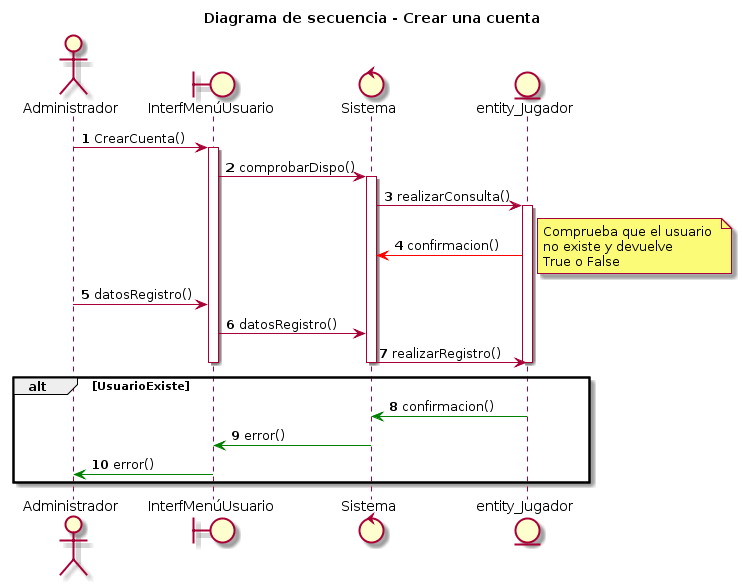
\includegraphics[width=1\textwidth]{./imatges/administrador/Crear_una_cuenta.png}
  \end{center}
  Para crear una cuenta, el administrador llama a la función CrearCuenta() a la Interfície del Menú del Usuario, el cual comprobará la disponibilidad, y el Sistema realiza una Consulta a la Entidad del Jugador para comprobar si el usuario ya existe o no. \\
  La confirmación que se envia al Sistema será True en el caso que se pueda crear la cuenta (el usuario no exista previamente) y False en el caso en el que el usuario ya esté registrado.
  \\
  
\subsubsection{Crear mapa}
\begin{center}
  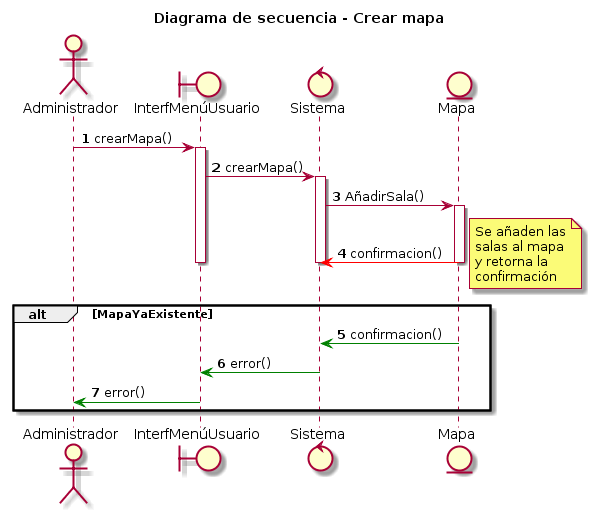
\includegraphics[width=1\textwidth]{./imatges/administrador/Crear_mapa.png}
  \end{center}
  
\subsubsection{Eliminar cuanta de usuario}
\begin{center}
  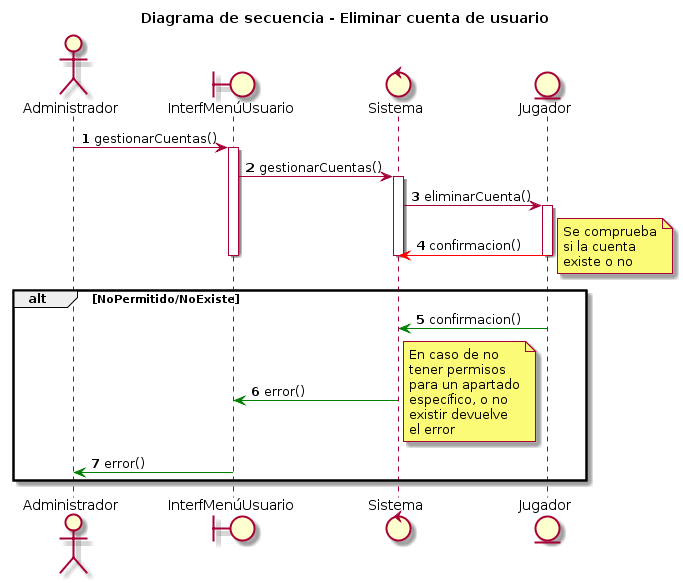
\includegraphics[width=0.9\textwidth]{./imatges/administrador/Eliminar_cuenta_de_usuario.png}
  \end{center}
  
\subsubsection{Modificar datos de la cuenta}
\begin{center}
  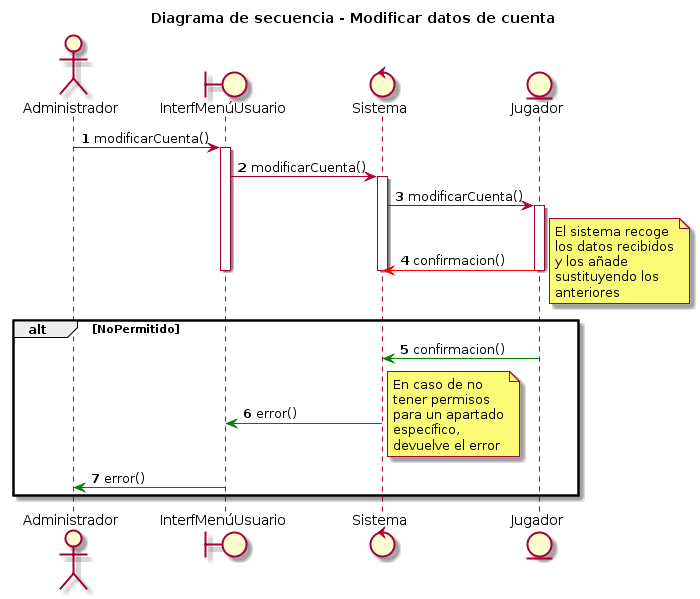
\includegraphics[width=0.9\textwidth]{./imatges/administrador/Modificar_datos_de_cuenta.png}
  \end{center}
  
\subsubsection{Modificar mapa}
\begin{center}
  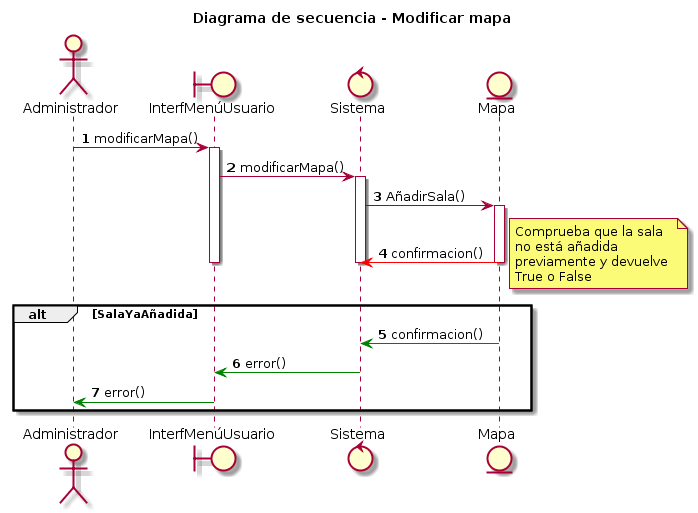
\includegraphics[width=0.9\textwidth]{./imatges/administrador/Modificar_mapa.png}
  \end{center}
  
\subsubsection{Modificar ranking}
\begin{center}
  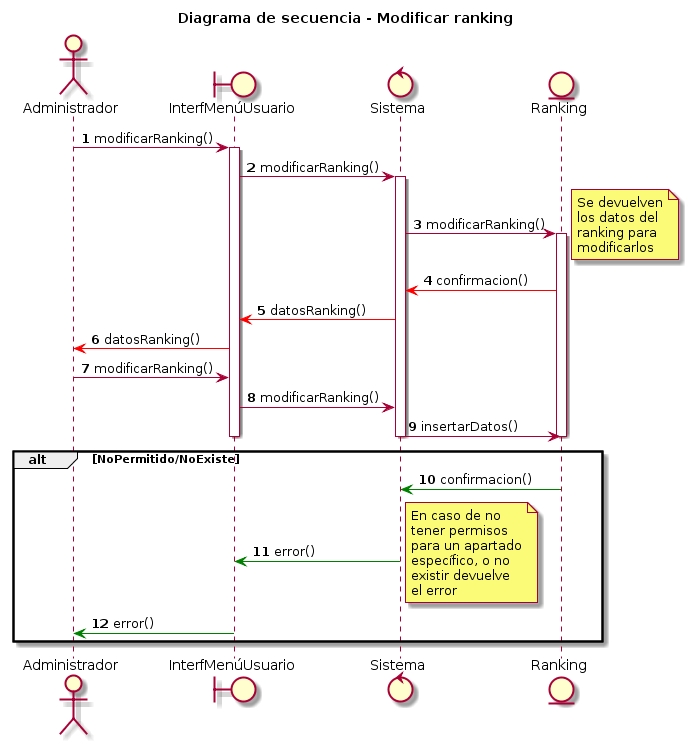
\includegraphics[width=0.9\textwidth]{./imatges/administrador/Modificar_ranking.png}
  \end{center}
  
\subsubsection{Ver usuarios en línea}
\begin{center}
  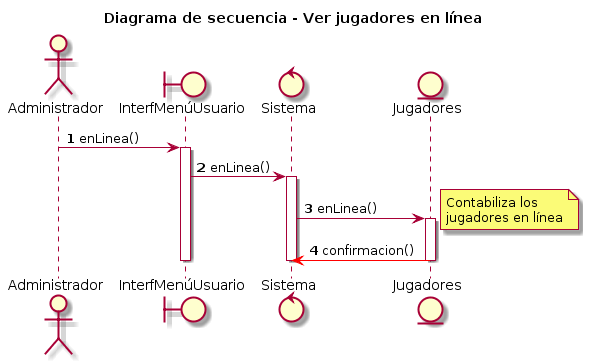
\includegraphics[width=0.9\textwidth]{./imatges/administrador/Ver_usuarios_en_linea.png}
  \end{center}



\subsection{Jugador}\label{sec:uc0}
\subsubsection{Consultar ranking}
\begin{center}
  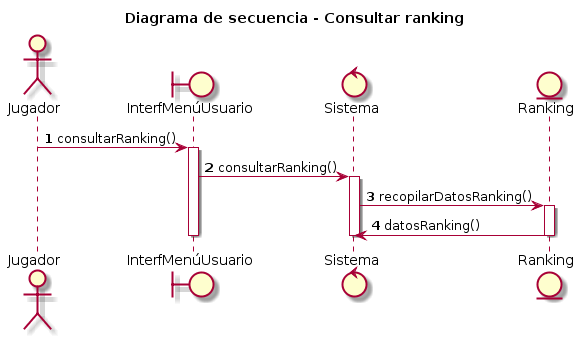
\includegraphics[width=0.9\textwidth]{./imatges/jugador/Consultar_ranking.png}
  \end{center}

\subsubsection{Continuar partida}
\begin{center}
  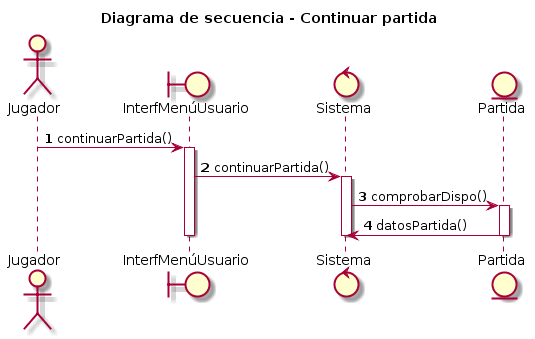
\includegraphics[width=0.9\textwidth]{./imatges/jugador/Continuar_partida.png}
  \end{center}
  
\subsubsection{Crear una cuenta}
\begin{center}
  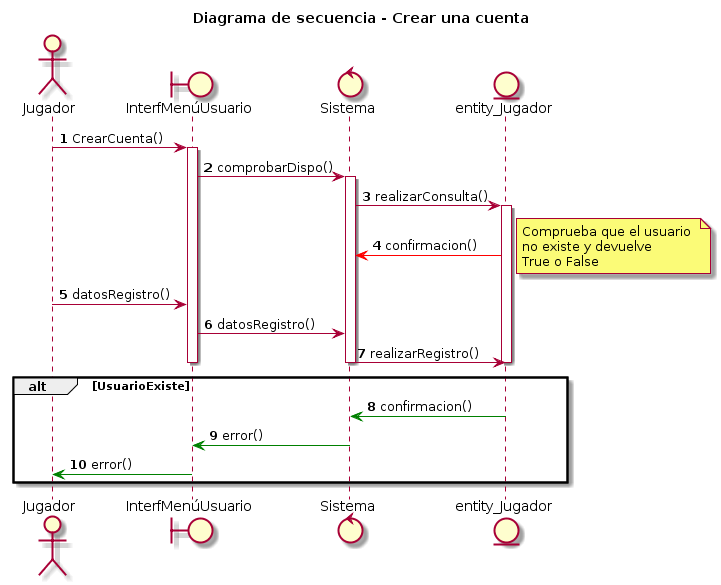
\includegraphics[width=0.9\textwidth]{./imatges/jugador/Crear_una_cuenta.png}
  \end{center}
  
\subsubsection{Eliminar partida}
\begin{center}
  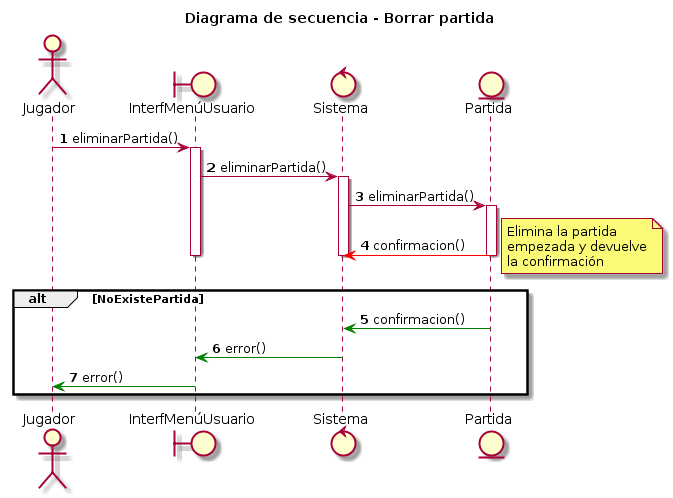
\includegraphics[width=0.9\textwidth]{./imatges/jugador/Eliminar_partida.png}
  \end{center}

\subsubsection{Empezar partida}
\begin{center}
  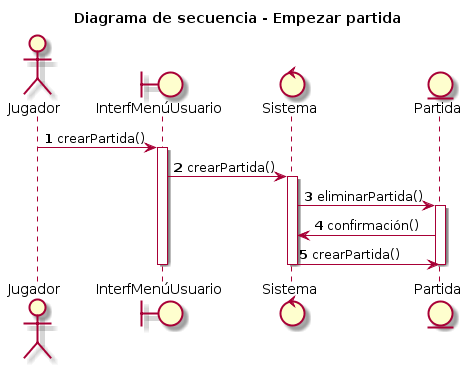
\includegraphics[width=0.9\textwidth]{./imatges/jugador/Empezar_partida.png}
  \end{center}

\subsubsection{Guardar partida}
\begin{center}
  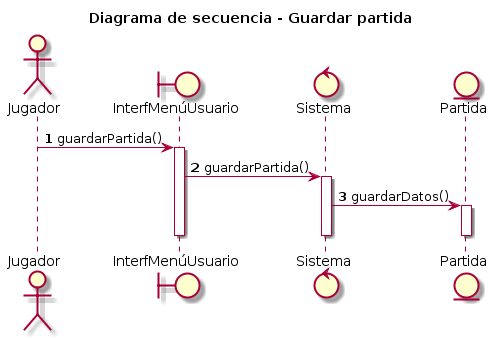
\includegraphics[width=0.9\textwidth]{./imatges/jugador/Guardar_partida.png}
  \end{center}

\subsubsection{Hacer login}
\begin{center}
  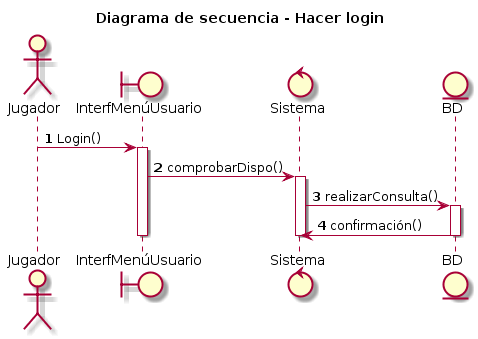
\includegraphics[width=0.9\textwidth]{./imatges/jugador/Hacer_login.png}
  \end{center}

\subsubsection{Menu de movimientos}
\begin{center}
  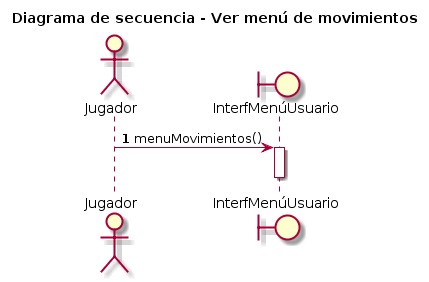
\includegraphics[width=0.9\textwidth]{./imatges/jugador/Menu_de_movimientos.png}
  \end{center}

\subsubsection{Modificar datos de la cuenta}
\begin{center}
  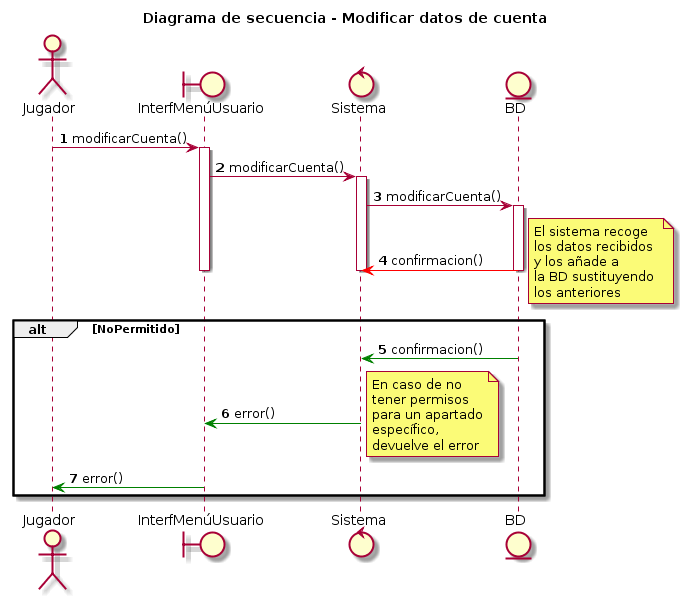
\includegraphics[width=0.9\textwidth]{./imatges/jugador/Modificar_datos_de_cuenta.png}
  \end{center}

\subsubsection{Salir del juego}
\begin{center}
  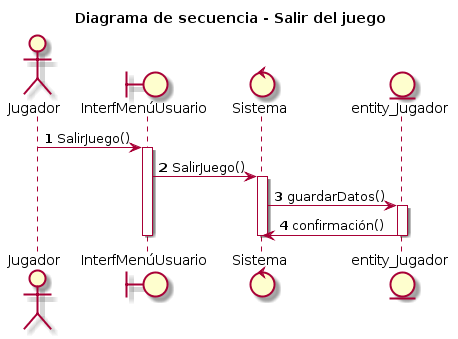
\includegraphics[width=0.9\textwidth]{./imatges/jugador/Salir_del_juego.png}
  \end{center}

